% !TEX program = xelatex
\documentclass[UTF8,a4paper,11pt,fontset=fandol]{ctexart}
\usepackage[left=25mm,right=23mm,top=25mm,bottom=24mm,headheight=16pt]{geometry}
\usepackage{amsmath,amssymb,booktabs,tabularx,longtable,array,multirow}
\usepackage{graphicx,float,xcolor,caption,enumitem,fancyhdr,setspace}
\usepackage{listings,xurl,hyperref,tikz}
\usetikzlibrary{positioning,arrows.meta,fit,calc}
\definecolor{forest}{HTML}{294C3B}
\definecolor{ink}{HTML}{26332C}
\definecolor{muted}{HTML}{687368}
\definecolor{paperline}{HTML}{D9DFD2}
\hypersetup{colorlinks=true,linkcolor=forest,citecolor=forest,urlcolor=forest,
 pdftitle={墒策：可信需水预测与灌溉决策——佐证材料},pdfauthor={得分队（AIC-2026-54247845）},bookmarksnumbered=true}
\setstretch{1.20}
\setlength{\parindent}{2em}
\setlength{\parskip}{.15em}
\setlength{\emergencystretch}{2em}
\ctexset{section={format=\Large\bfseries\color{forest},beforeskip=1.2em,afterskip=.8em},
 subsection={format=\large\bfseries\color{forest},beforeskip=1em,afterskip=.5em},
 subsubsection={format=\normalsize\bfseries,beforeskip=.8em,afterskip=.4em}}
\captionsetup{font=small,labelfont=bf,skip=7pt}
\setlist{nosep,leftmargin=2em}
\renewcommand{\arraystretch}{1.22}
\pagestyle{fancy}\fancyhf{}
\fancyhead[L]{\small\color{muted}墒策\quad 佐证材料}
\fancyhead[R]{\small\color{muted}AI＋农业}
\fancyfoot[C]{\small\thepage}
\renewcommand{\headrulewidth}{.3pt}
\newcommand{\ET}{\mathrm{ET}_{0}}
\newcommand{\MAE}{\operatorname{MAE}}
\newcommand{\RMSE}{\operatorname{RMSE}}
\newcommand{\clip}{\operatorname{clip}}
\newcommand{\file}[1]{\texttt{\small\path{#1}}}
\newcommand{\datafigure}[4][.94]{\begin{figure}[H]\centering\includegraphics[width=#1\linewidth]{figures/#2}\caption{#3}\label{#4}\end{figure}}
\newcommand{\datatable}[4]{\begin{table}[H]\centering\small\caption{#2}\label{#3}\input{tables/#1}\par\vspace{4pt}{\footnotesize\color{muted}#4}\end{table}}
\lstset{basicstyle=\ttfamily\footnotesize,breaklines=true,columns=fullflexible,
 frame=single,rulecolor=\color{paperline},backgroundcolor=\color{white},showstringspaces=false}
\begin{document}
\thispagestyle{empty}
\begin{center}
{\Large\bfseries\color{forest} 墒策：可信需水预测与灌溉决策\par}\vspace{2mm}
{\LARGE\bfseries 佐证材料\par}\vspace{3mm}
{\color{muted} 团队名称：得分队\qquad 团队编号：AIC-2026-54247845\qquad 赛题：AI＋农业\par}
\end{center}
\vspace{2mm}{\color{forest}\rule{\linewidth}{.8pt}}

本材料汇总作品真实性与有效性的证据：数据来源及授权、数据完整性校验、模型训练与测试记录、软件测试记录、系统运行截图和实际决策记录样例。所有记录均可在完整工程中由对应脚本重新生成。

\section*{1\quad 数据来源与使用授权}
\begin{itemize}
\item \textbf{数据来源}：Open-Meteo历史天气接口（\url{https://open-meteo.com/en/docs/historical-weather-api}），模式ERA5，时区Asia/Shanghai，时间范围2018-01-01至2025-12-31。
\item \textbf{使用授权}：Open-Meteo接口数据采用CC BY 4.0许可（\url{https://open-meteo.com/en/licence}），允许在署名条件下使用与再分发，本作品在技术方案、系统界面与本材料中均已署名。
\item \textbf{方法依据}：FAO-56作物蒸散与灌溉需水计算方法（Allen等，1998）；共形预测方法（Vovk等，2005；Lei等，2018）。
\end{itemize}

\begin{table}[H]\centering\small\caption{三地数据完整性检查}
\begin{tabular}{lrrcr}\toprule
地点 & 逐日记录 & 缺失单元 & 返回网格（纬度, 经度） & 网格海拔\\\midrule
石家庄 & 2922 & 0 & 38.00, 114.50 & 77 m\\
郑州 & 2922 & 0 & 34.75, 113.50 & 110 m\\
济南 & 2922 & 0 & 36.75, 117.00 & 136 m\\
\bottomrule\end{tabular}\end{table}

\begin{table}[H]\centering\small\caption{原始接口响应的SHA-256校验值（工程中\texttt{inputs/provenance.json}）}
\begin{tabular}{ll}\toprule 文件 & SHA-256\\\midrule
\file{inputs/weather/shijiazhuang.json} & \texttt{\scriptsize 930964d6fa3b8ce4b6e180b4ba6fb5579d6a007ea6145ebba4b8bb28ac79c30a}\\
\file{inputs/weather/zhengzhou.json} & \texttt{\scriptsize a6f27b8630a2487596d48965a3df36309e3eb7271252f6aac5b805a56cdbea9d}\\
\file{inputs/weather/jinan.json} & \texttt{\scriptsize 123e9a9e5b6ca60c46f7a20017684928e46746943eb630bfa662ca5f3480a35d}\\
\bottomrule\end{tabular}\end{table}

\section*{2\quad 模型训练与测试记录}
\begin{table}[H]\centering\small\caption{模型运行记录（\texttt{results/summary.json}）}
\begin{tabular}{ll}\toprule 项目 & 记录\\\midrule
运行环境 & Python 3.12.14 · NumPy 2.2.6 · pandas 2.3.3 · scikit-learn 1.7.2\\
训练 / 校准 / 测试样本 & 5457 / 1095 / 2193（按年份切分）\\
训练截止 / 校准截止 & 2022-12-31 / 2023-12-31\\
测试MAE / RMSE / $R^2$ & 0.775680 / 1.068795 / 0.710346\\
昨日值基线MAE & 0.840251（降低7.6847\%）\\
90\%区间半宽$q$ / 测试覆盖率 & 1.850583 mm/日 / 91.0625\%\\
MAE差值95\%区间（块自助） & [0.0332, 0.0965] mm/日\\
单次推理中位耗时 & 11.5 ms（50次单行推理）\\
策略仿真 & 180组生长季，27540条逐日水量记录\\\bottomrule
\end{tabular}\end{table}

\section*{3\quad 软件测试记录}
\begin{table}[H]\centering\small\caption{核心单元测试（\texttt{tests/test\_core.py}，9项全部通过）}
\begin{tabularx}{\linewidth}{@{}p{.36\linewidth}X@{}}\toprule 测试 & 检查内容\\\midrule
FAO-56参考蒸散公式 & 程序实现与逐项标量计算结果一致（误差小于$10^{-10}$）\\
未来数据泄漏 & 扰动目标日及之后的全部气象数据，49维输入特征不变\\
水量守恒 & 日末亏缺、排水与未满足需水满足守恒关系\\
触发边界与供水上限 & 恰在阈值不灌溉、越过阈值触发；建议量不超过日上限\\
异常输入（4项） & 负值、超过TAW、NaN、无穷大等亏缺输入被拒绝\\
共形次序统计量 & 有限样本分位数序号与取值计算正确\\\bottomrule
\end{tabularx}\end{table}

\begin{table}[H]\centering\small\caption{浏览器端自动化测试（\texttt{scripts/browser\_check.cjs}，9项全部通过）}
\begin{tabular}{rll}\toprule 序号 & 检查项 & 结果\\\midrule
1 & 页面加载后完成模型推理并给出建议 & 通过\\
2 & 供水上限过小时显示能力不足提示 & 通过\\
3 & 导出JSON与页面当前输入一致 & 通过\\
4 & 模型验证表正确渲染 & 通过\\
5 & 策略回测表正确渲染 & 通过\\
6 & 非法输入时禁止导出 & 通过\\
7 & 修正参数后恢复计算 & 通过\\
8 & 手机竖屏无横向溢出 & 通过\\
9 & 全程无未捕获脚本错误 & 通过\\
\bottomrule\end{tabular}\end{table}

交付核验脚本\file{scripts/verify_delivery.py}从CSV重新计算全部模型指标与覆盖率，将27540条逐日记录汇总后与180组季节结果逐项比对，并校验原始数据哈希、PDF与PPTX文件完整性、视频时长与可解码性，全部通过。

\section*{4\quad 系统运行截图}
\begin{figure}[H]\centering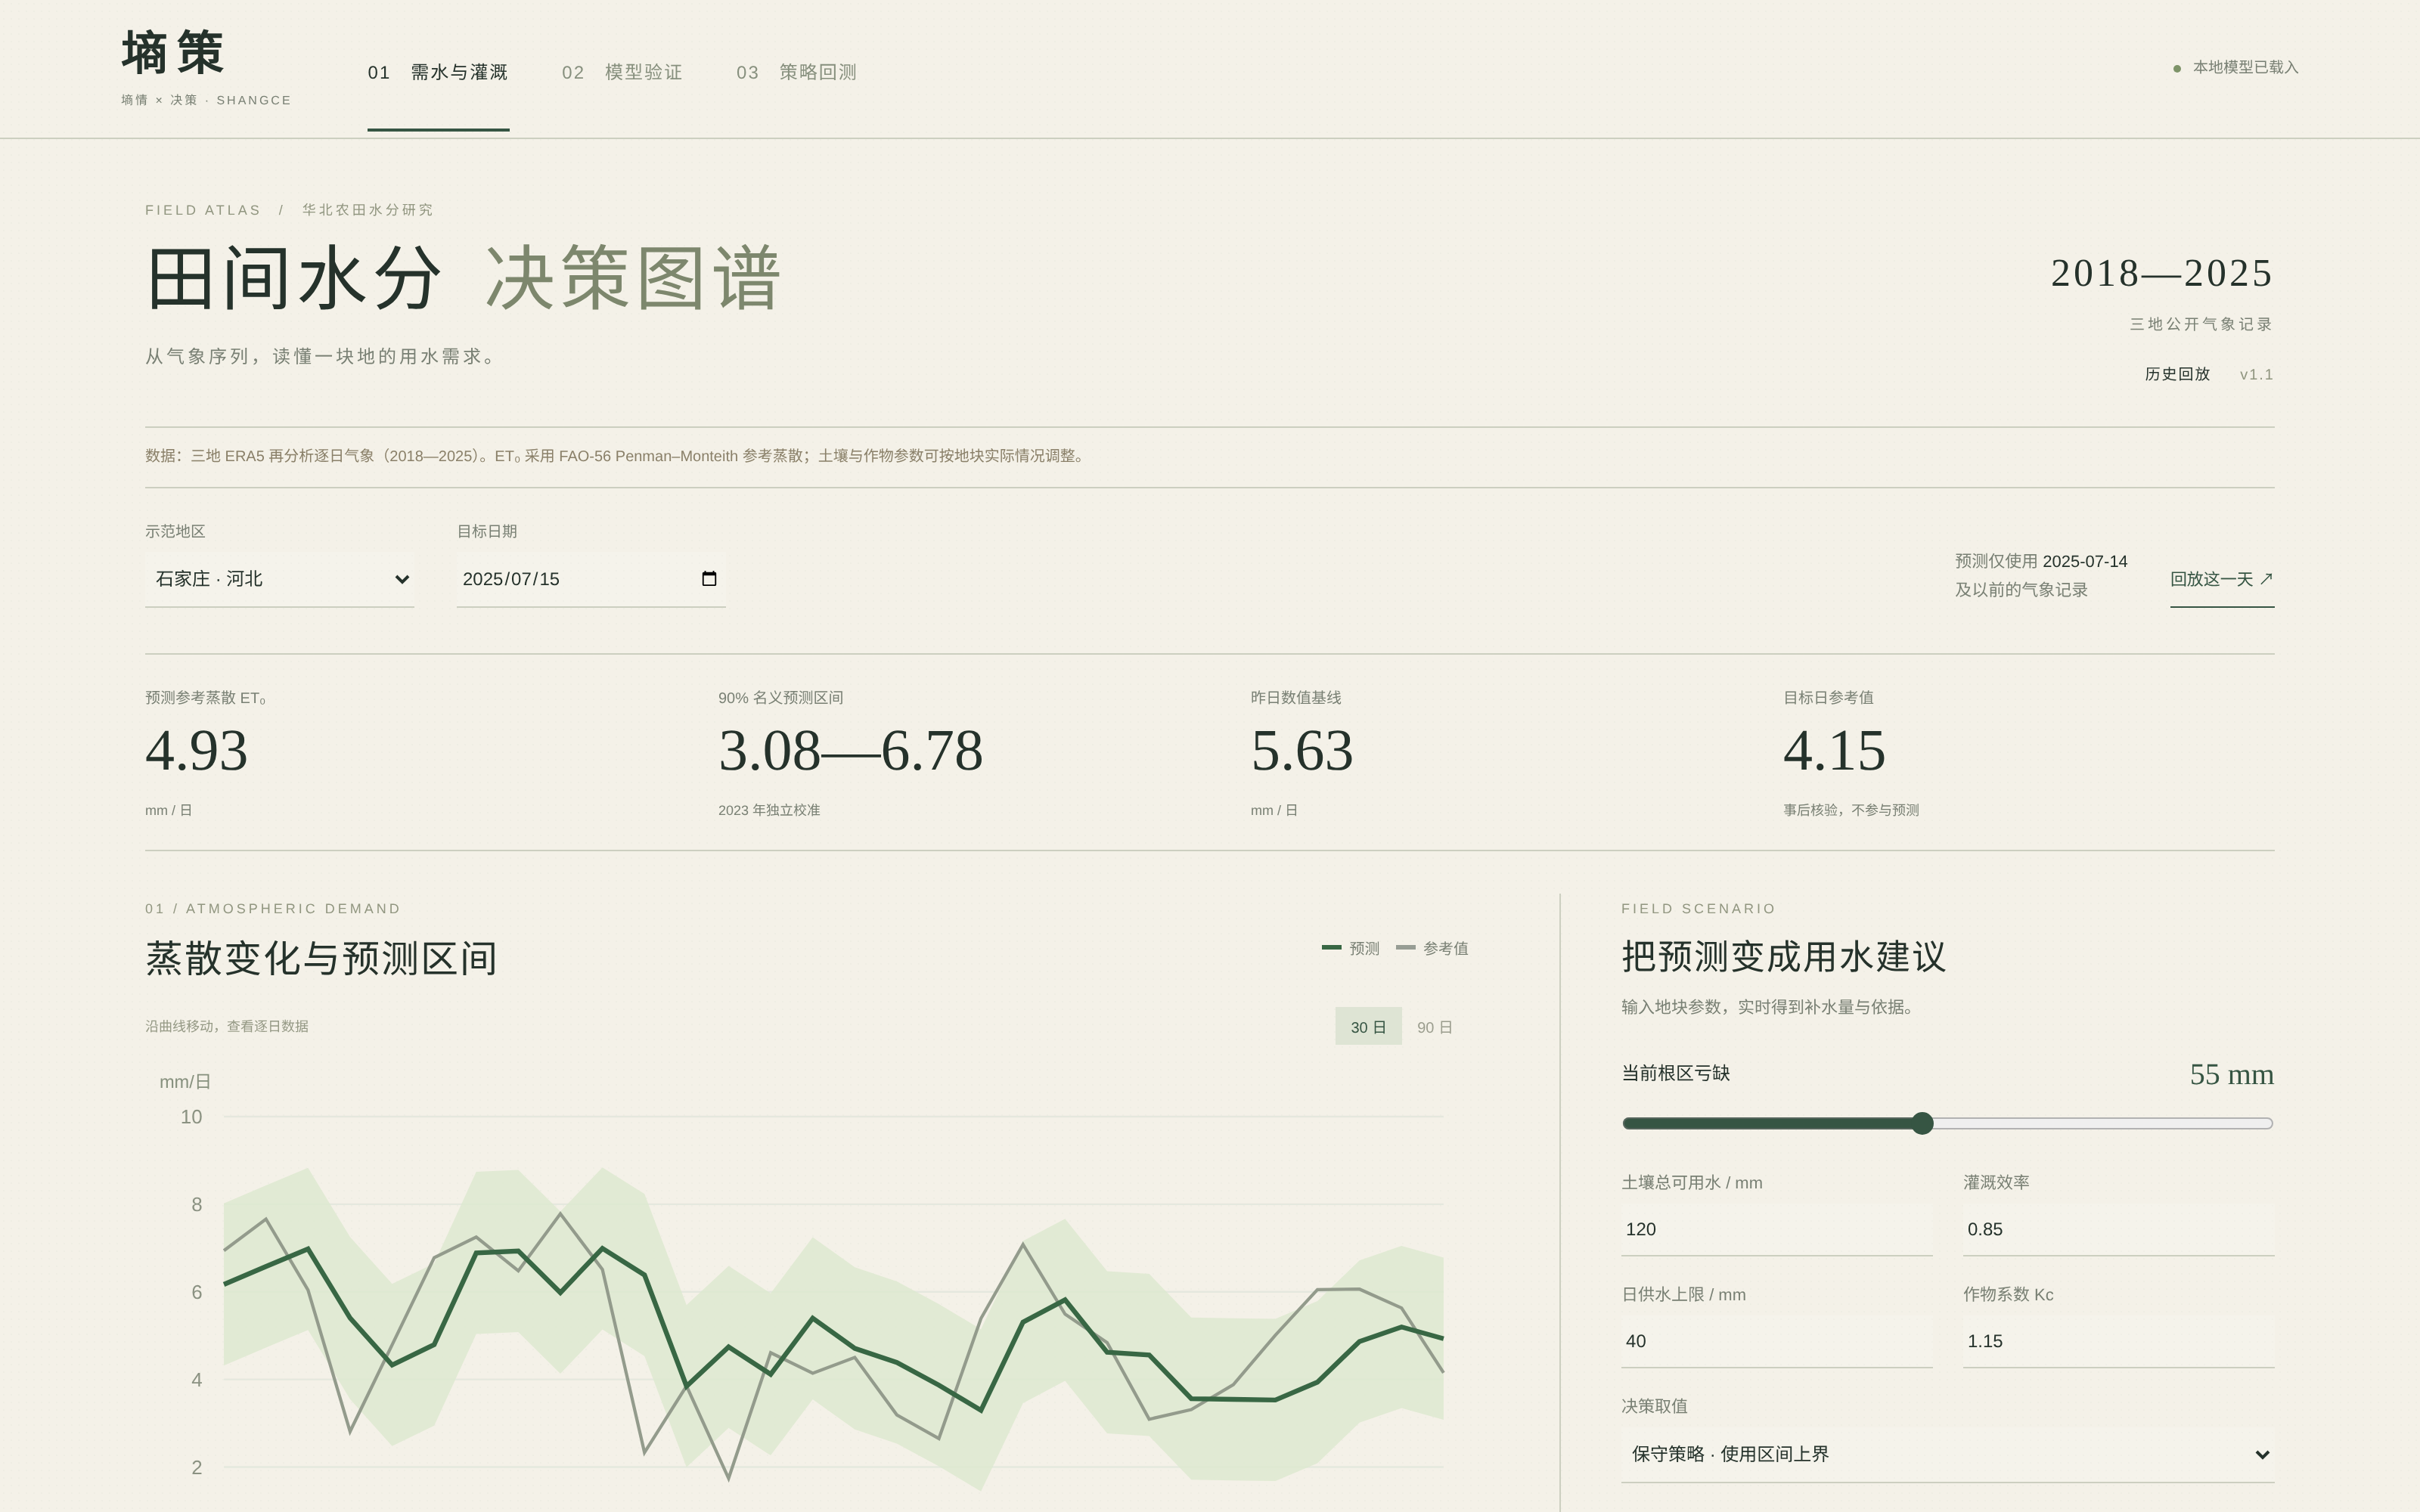
\includegraphics[width=\linewidth]{../results/screenshots/dashboard.png}
\caption{需水与灌溉视图：石家庄2025年7月15日的次日需水预测、90\%区间与灌溉建议}\end{figure}
\begin{figure}[H]\centering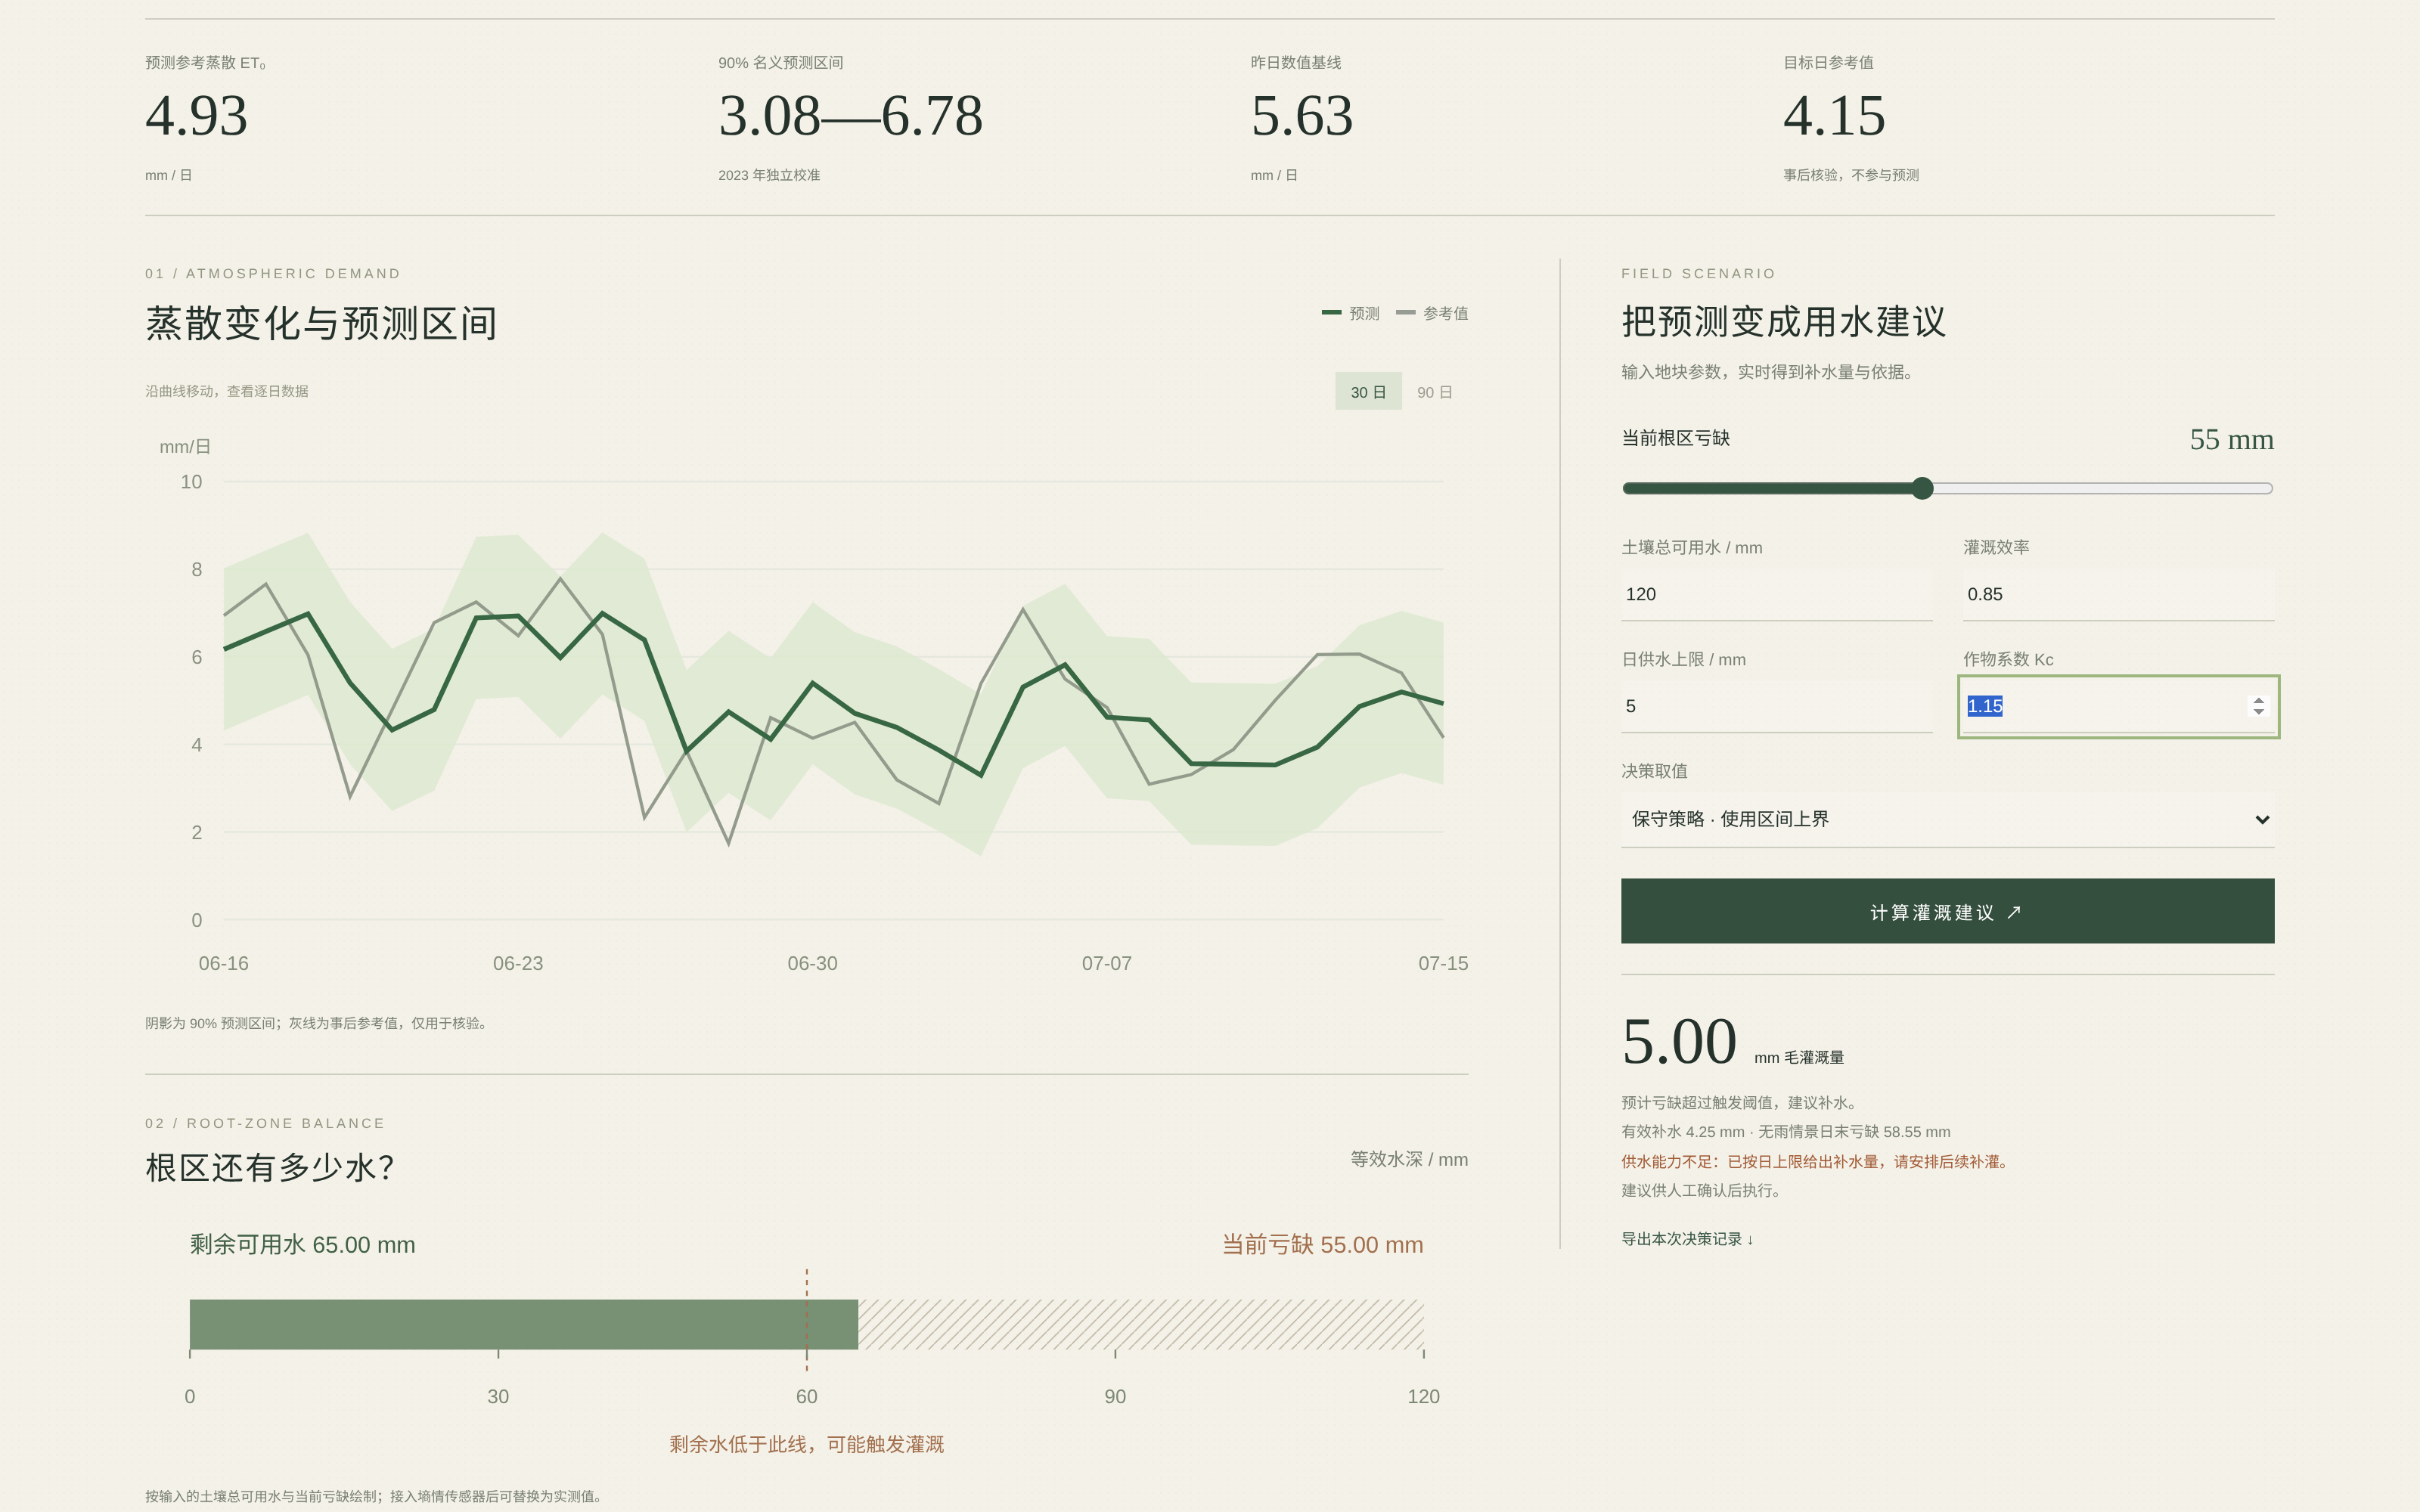
\includegraphics[width=\linewidth]{../results/screenshots/capacity.png}
\caption{日供水上限设为5 mm时，系统按上限给出补水量并提示供水能力不足}\end{figure}
\begin{figure}[H]\centering
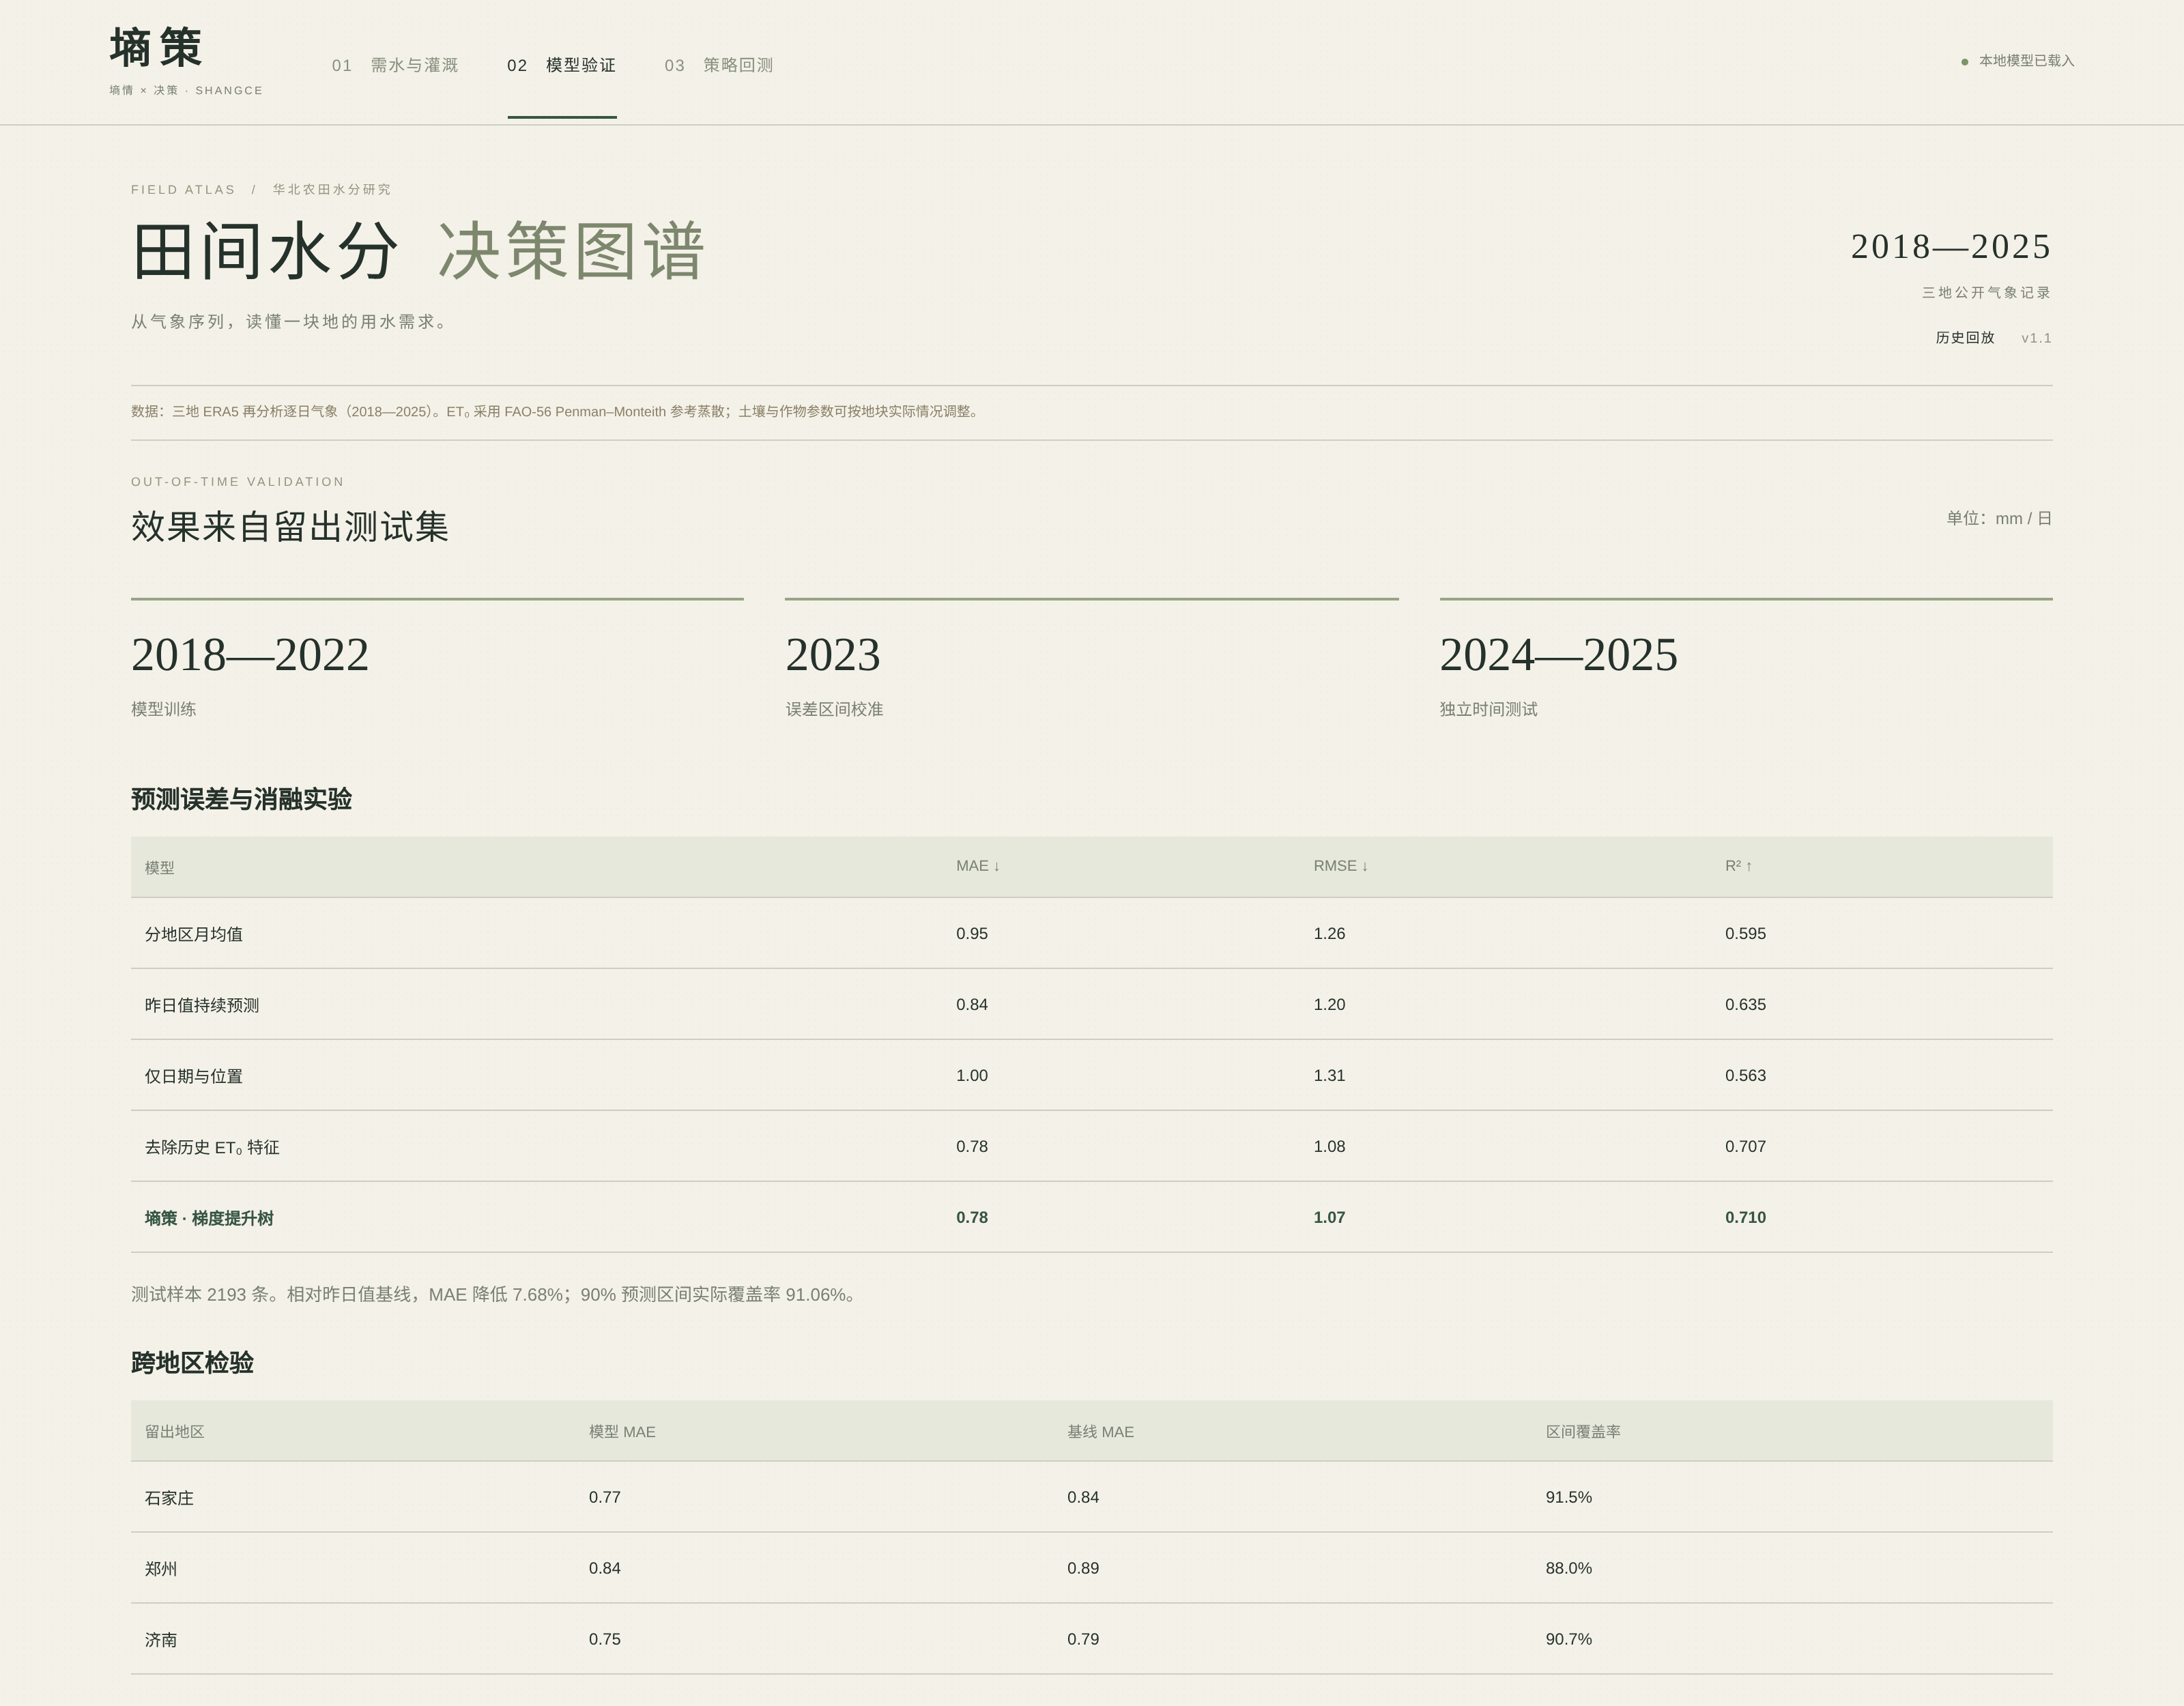
\includegraphics[width=.49\linewidth]{../results/screenshots/evidence_view.png}\hfill
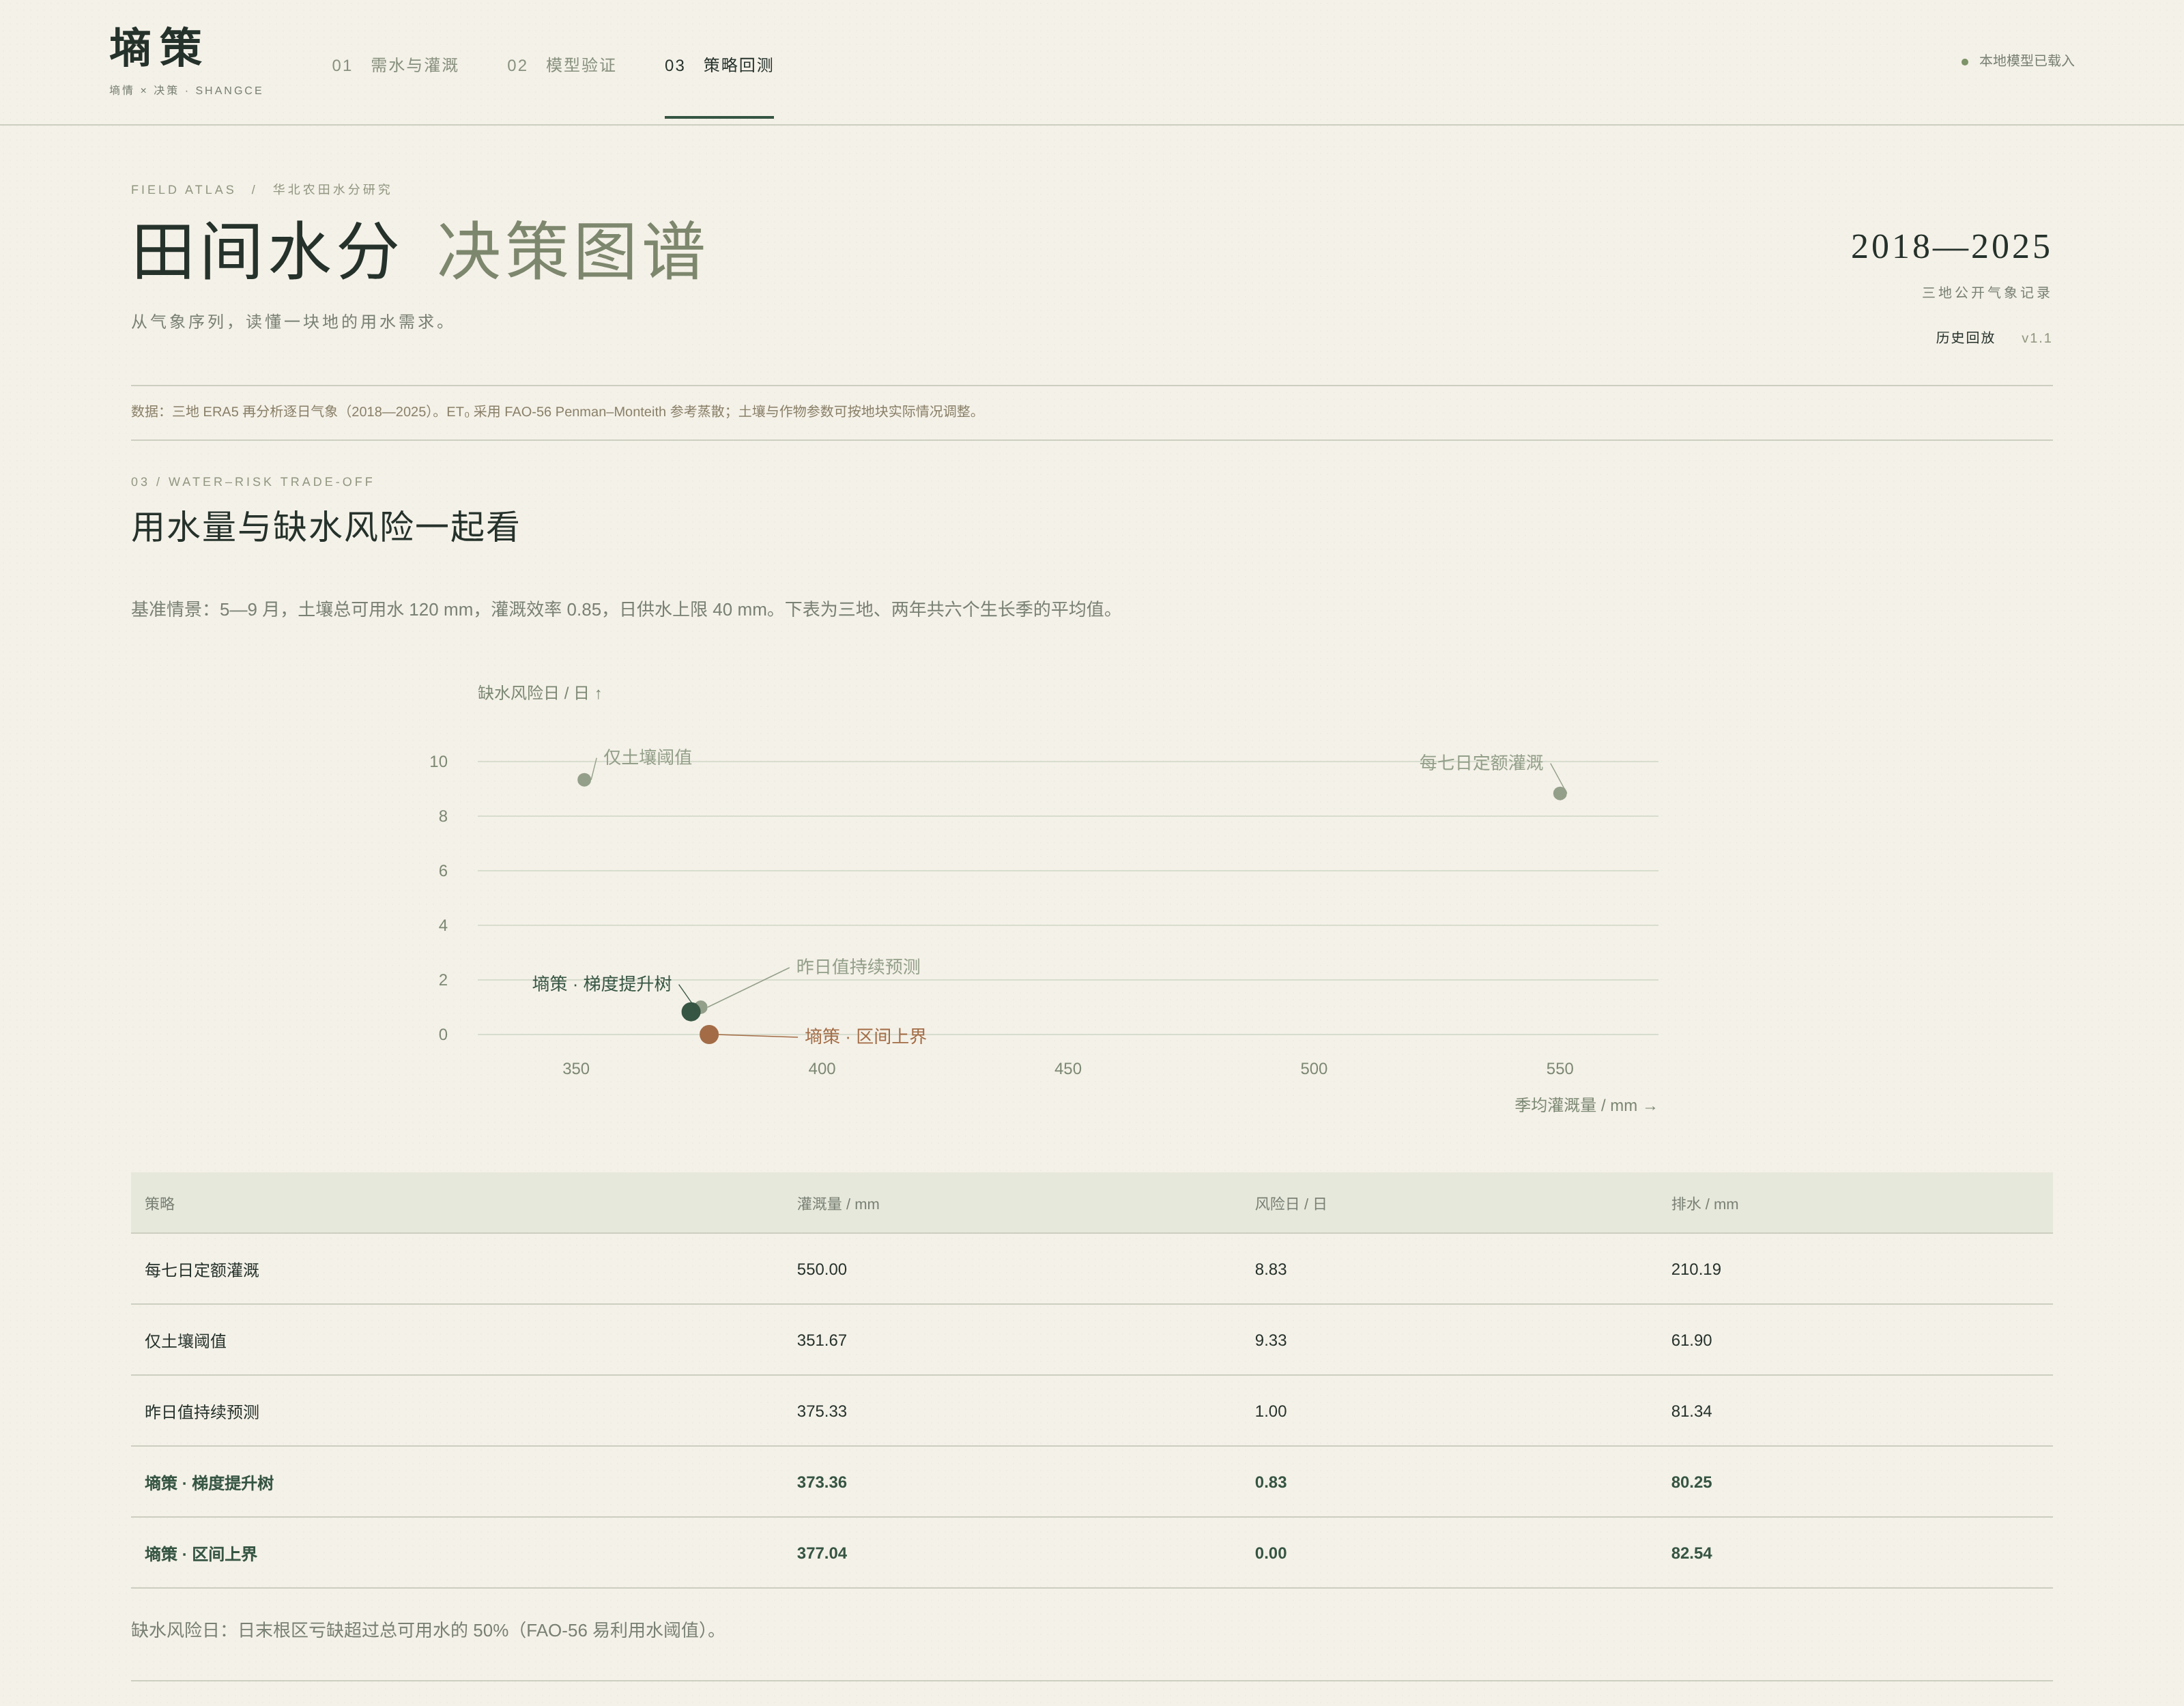
\includegraphics[width=.49\linewidth]{../results/screenshots/simulation_view.png}
\caption{模型验证视图（左）与策略回测视图（右）}\end{figure}
\begin{figure}[H]\centering
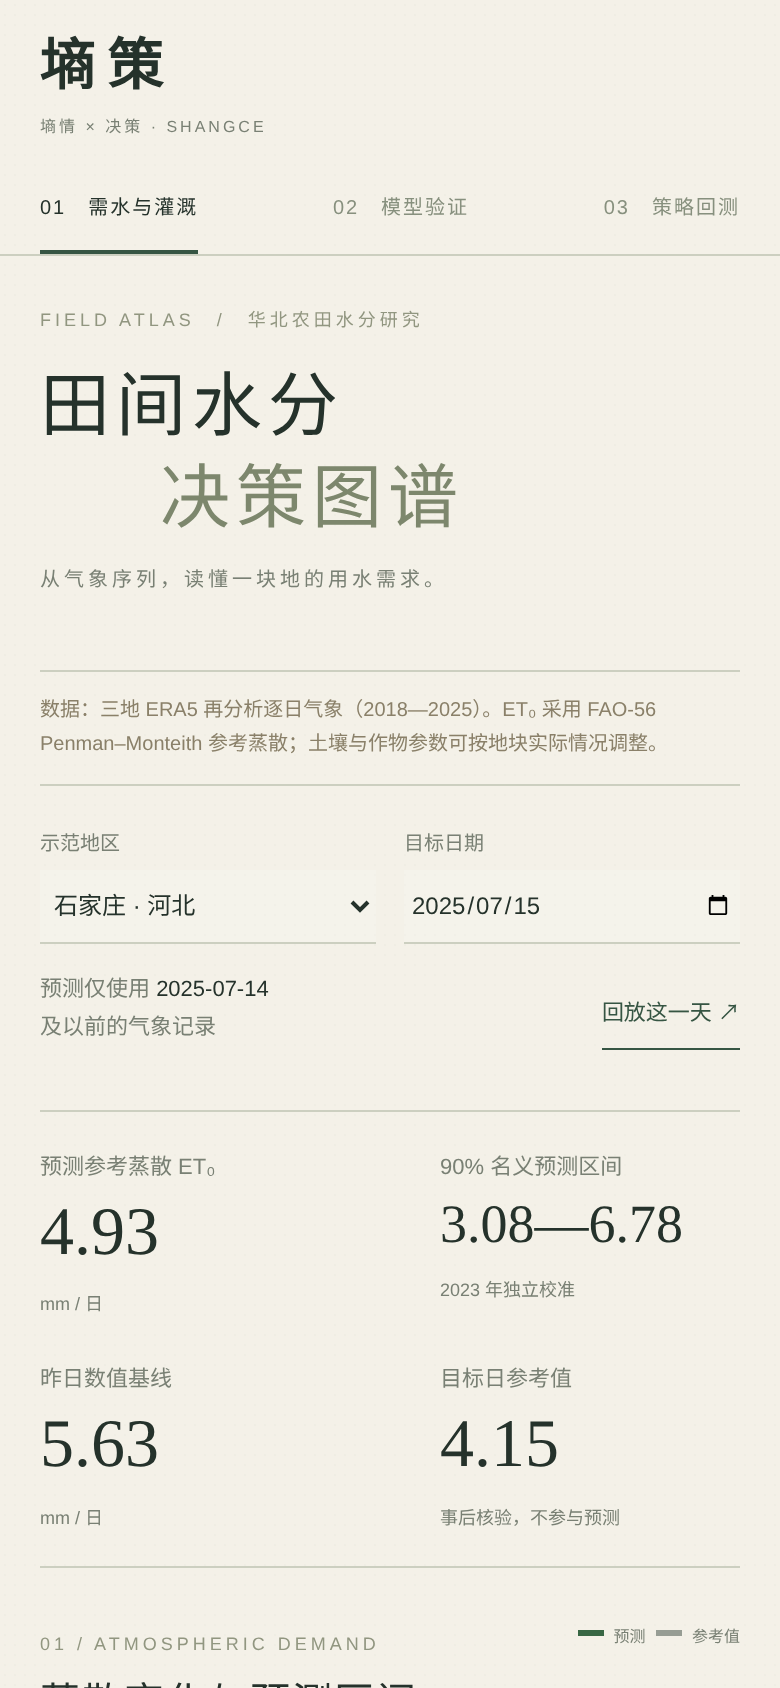
\includegraphics[height=.36\textheight]{../results/screenshots/mobile.png}
\caption{手机端界面（竖屏无横向溢出）}\end{figure}

\section*{5\quad 决策记录样例}
以下为系统导出的一条实际决策记录（\file{results/sample_decision.json}，节选）。济南2025年7月15日，采用区间上界策略，当前亏缺90 mm、日供水上限5 mm，系统给出5 mm毛灌溉量并标记供水受限，计算过程见技术方案附录。
\begin{lstlisting}
{
  "site": "jinan", "date": "2025-07-15", "mode": "upper",
  "mean_et0_mm": 6.1737, "upper_et0_mm": 8.0243,
  "inputs": {"deficit": 90, "taw": 120, "eta": 0.85, "cap": 5, "kc": 1.15},
  "triggered": true, "gross_mm": 5, "net_mm": 4.25,
  "projected_deficit_mm": 94.978, "capacity_limited": true,
  "model_train_end": "2022-12-31", "calibration_end": "2023-12-31"
}
\end{lstlisting}
\end{document}
